\chapter{Dịch máy bằng mô hình học LSTM-Attention}
\ifpdf
    \graphicspath{{Chapter3/Chapter3Figs/PNG/}{Chapter3/Chapter3Figs/PDF/}{Chapter3/Chapter3Figs/}}
\else
    \graphicspath{{Chapter3/Chapter3Figs/EPS/}{Chapter3/Chapter3Figs/}}
\fi
\label{chap_3}
\begin{quote}
\textit{Chương này trình bày về việc tổ chức các LSTM theo kiến trúc Bộ mã hóa-Bộ giải mã cùng với sử dụng cơ chế Attention. Ở đây, chúng tôi tập trung tìm hiểu về LSTM trong kiến trúc Bộ mã hóa-Bộ giải mã và các phiên bản của cơ chế Attention, sau đó giải thích chúng dựa trên cơ sở Toán học. Cụ thể, về LSTM, chúng tôi sử dụng bi-LSTM và uni-LSTM, về Attention, chúng tôi tìm hiểu về hai phiên bản Toàn cục (Global) và Cục bộ (Local):
\begin{itemize}
	\item LSTM: chúng tôi tổ chức các bi-LSTM và uni-LSTM theo kiến trúc Bộ mã hóa-Bộ giải mã để tránh được hạn chế về số lượng từ ở ngôn ngữ nguồn và ngôn ngữ đích.
	\item Attention: chúng tôi tìm hiểu được sự hạn chế hiện có của kiến trúc Bộ mã hóa-Bộ giải mã khi thực hiện dịch những câu dài. Do vậy, chúng tôi sử dụng cơ chế Attention để giải quyết hạn chế đó bằng cách sử dụng thêm các trạng thái ẩn của bộ mã hóa trong quá trình giải mã.
	\begin{itemize}
		\item Toàn cục: phiên bản này sử dụng tất cả trạng thái ẩn trong bộ mã hóa trong quá trình giải mã.
		\item Cục bộ: phiên bản này chỉ sử dụng một số trạng thái ẩn trong bộ mã hóa trong quá trình giải mã.
	\end{itemize}
\end{itemize}}
\end{quote}
\section{LSTM với kiến trúc Bộ mã hóa-Bộ giải mã}
Hạn chế của việc sử dụng một mô hình LSTM khi áp dụng vào trong bài toán Dịch máy là ràng buộc chiều dài của câu đầu vào (ngôn ngữ nguồn) phải bằng chiều dài của câu đầu ra (ngôn ngữ đích). Bởi vì tại mỗi thời điểm, LSTM nhận đầu vào là một từ ở ngôn ngữ nguồn, sau đó thực hiện dự đoán một từ ở ngôn ngữ đích. Do vậy, một mô hình LSTM chỉ có thể dịch ổn trên những cặp ngôn ngữ rất giống nhau (ví dụ như Trung-Việt) nhưng chất lượng dịch vẫn rất khó đảm bảo vì thậm chí giữa cặp ngôn ngữ này dù rất giống nhau nhưng vẫn có cách diễn đạt, sử dụng từ ngữ khác nhau. // TODO: Đưa ra ví dụ. Dễ nhận thấy rằng đây là một giả định phi thực tế, dẫu là con người dịch thì cũng rất khó và phải là người am hiểu về cả 2 ngôn ngữ đó thì mới có thể dịch sang ngôn ngữ đích mà vẫn truyền đạt được đẩy đủ ý nghĩa ở ngôn ngữ nguồn. Đối với ràng buộc chiều dài ở 2 câu phải bằng nhau thì chỉ phù hợp với khi dịch thơ có luật ràng buộc về số từ như thơ lục bát, thơ Đường v.v... Tuy nhiên, dù đã thỏa ràng buộc về số lượng từ nhưng vẫn khó đảm bảo về mặt ngữ nghĩa. Trong thơ văn, người ta sử dụng rất nhiều biện pháp tu từ, văn phong và ngữ pháp thì rất đa dạng, cách hành văn rất khác. Hơn nữa, một câu có thể biểu diễn bởi rất nhiều cách khác nhau. Minh chứng là một bài thơ tiếng Trung có thể có rất nhiều bản dịch khác nhau. Từ những lí do kể trên, sử dụng một mô hình LSTM để giải quyết bài toán Dịch máy là không phù hợp với thực tế. 

Để giải quyết những hạn chế của đó, nhóm tác giả Sutskever, 2014 \cite{Seq2Seq2014} đã đề xuất một kiến trúc tên gọi là Chuỗi tới Chuỗi (Sequence to Sequence - Seq2Seq). Tuy nhiên, mọi người thường gọi kiến trúc này là kiến trúc Bộ mã hóa-Bộ giải mã (Encoder-Decoder). Trong khóa luận này, chúng tôi sử dụng kiến trúc này để giải quyết bài toán Dịch máy và gọi nó là Bộ mã hóa-Bộ giải mã. Ý tưởng của kiến trúc này rất đơn giản. Kiến trúc này tận dụng các đặc tính của các mô hình LSTM và tổ chức chúng một cách hợp lí sao cho phù hợp với các yêu cầu của bài toán Dịch máy. 

Kiến trúc Bộ mã hóa-Bộ giải mã như tên gọi, gồm có 2 bộ phận chính là bộ mã hóa và bộ giải mã. Mỗi một bộ phận sẽ là một mô hình học được lựa chọn sao cho phù hợp với bài toán và có thể hoạt động tốt với nhau. Đối với bài toán Dịch máy và trong phạm vi khóa luận này, mỗi bộ phận sẽ là một mạng nơ-ron hồi qui, cụ thể là các LSTM. 

\begin{figure}
	\centering
	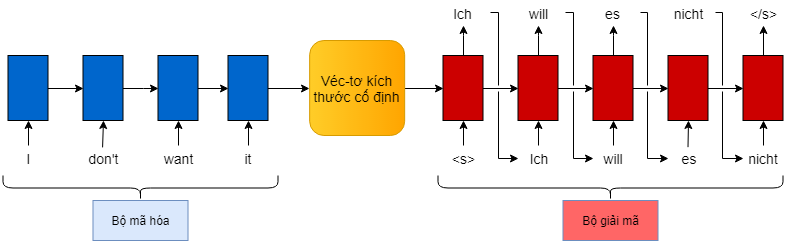
\includegraphics[width=0.8\textwidth]{Encoder-Decoder_2}
	\caption[Minh họa kiến trúc Bộ mã hóa-Bộ giải mã.]{Minh họa kiến trúc Bộ mã hóa-Bộ giải mã. Kiến trúc có 2 bộ phận. Trong đó, bộ mã hóa là một bi-LSTM có nhiệm vụ nhận câu nguồn làm đầu vào và xuất ra một véc-tơ có kích thước cố định chứa thông tin cần thiết để dịch của toàn bộ câu nguồn. Bộ giải mã là một uni-LSTM có đầu vào là véc-tơ có kích thước cố định của bộ mã háo và đầu ra là câu đích.}
	\label{fig_Encoder-Decoder}
\end{figure}

Hình \ref{fig_Encoder-Decoder} minh họa kiến trúc Bộ mã hóa-Bộ giải mã trong việc giải quyết bài toán Dịch máy. Chúng tôi sẽ trình bày cụ thể về cách hoạt động của 2 bộ phận này trong các phần tiếp theo.

\subsection{Bộ mã hóa}
Bộ mã hóa là một bi-LSTM (LSTM 2 chiều). Bi-LSTM này nhận đầu vào là một câu ở ngôn ngữ nguồn $\bm{x} = \{x_0, ..., x_{S-1}\}$. Đầu ra là một véc-tơ có kích thước cố định. Véc-tơ này chứa các thông tin cần thiết để tiến hành dịch sang câu ở ngôn ngữ đích. Nhiệm vụ của bộ mã hóa (Bi-LSTM) là thực hiện mã hóa toàn bộ câu nguồn thành véc-tơ có chứa các thông tin hữu ích. Véc-tơ kích thước cố định này rất quan trọng, nó là tiền đề để việc dịch sang câu đích đạt chất lượng tốt.

Ở đây, chúng tôi sử dụng véc-tơ trạng thái ẩn $h_t$ làm véc-tơ có kích thước cố định. Lí do bởi vì trong Bi-LSTM, trạng thái ẩn của một từ thứ $t$ (thời điểm $t$) chứa những thông tin, mối quan hệ giữa từ này và những từ lân cận. Hơn nữa, nó còn chứa thông tin của toàn bộ những từ ở đầu câu cho tới từ thứ $t$. Vậy nên trạng thái ẩn của từ cuối cùng của câu sẽ chứa đựng thông tin của toàn bộ những từ trong câu. Và điều đó phù hợp với ý tưởng của véc-tơ có kích thước cố định của bộ mã hóa. 

Trong thực tế, đầu ra của bộ mã hóa có thể là bất kì véc-tơ có tính chất như thế nào. Trong một số công trình sử dụng thêm một phép biến đổi trên trạng thái ẩn cuối cùng của bi-LSTM để tạo ra một véc-tơ có kích thước cố định. Đối với bài toán như Phát sinh câu miêu tả cho ảnh, đầu ra của bộ mã hóa là một véc-tơ kích thước cố định chứa đặc trưng hữu ích của toàn bộ bức ảnh.


\subsection{Bộ giải mã}
Bộ giải mã là một uni-LSTM (LSTM 1 chiều). Uni-LSTM này nhận đầu vào là một véc-tơ kích thước cố định chứa thông tin cần thiết của câu cần dịch. Véc-tơ này là véc-tơ kích thước cố định từ đầu ra của bộ mã hóa. Đầu ra của bộ giải mã là câu đã được dịch sang ngôn ngữ đích $\bm{y} = \{y_0, ..., y_{S-1}\}$.
Lí do chúng tôi sử dụng uni-LSTM mà không phải là bi-LSTM bởi vì trong quá trình giải mã (dịch) mô hình chỉ biết có được những từ đã được dịch ở trước đó (thông tin trong quá khứ) mà không biết được những từ đằng sau (thông tin trong tương lai) (vì chưa được dịch). Do đó, việc sử dụng lợi thế của bi-LSTM trong bộ giải mã là không thể và có thể gây ảnh hưởng tới chất lượng dịch của mô hình.

Một điều đáng lưu ý trong việc huấn luyện uni-LSTM trong bộ giải mã là đầu vào của uni-LSTM trong mỗi thời điểm $t$. Hình \ref{fig_Encoder-Decoder} minh họa bộ giải mã trong quá hình kiểm thử. Từ được dự đoán ở thời điểm $t-1$ sẽ là đầu vào của uni-LSTM ở thời điểm $t$. Tuy nhiên, việc như vậy sẽ là hạn chế lớn nếu sử dụng nó trong quá trình huấn luyện. Tại mỗi thời điểm $t$, khi thực hiện dự đoán từ đích tiếp theo, mô hình sẽ dựa vào những từ ở phía trước rồi sau đó sẽ tính độ lỗi dựa trên từ đúng được cung cấp. Do vậy, việc dự đoán tại thời điểm $t$ có tốt hay không còn cần phải xem những từ đã được dự đoán ở phía trước có tốt hay không nữa. Nếu những từ ban đầu dự đoán không tốt, tất cả những được dự đoán ở phía sau sẽ càng kém hơn nữa. Để mô hình có thể học được cách dịch một câu dài với quá trình huấn luyện như trên thì phải tốn nhiều thời gian. Vì vậy, chúng tôi sử dụng phương pháp huấn luyện mạng nơ-ron hồi quy hiệu quả là \textit{teacher forcing} // TODO: dịch. Phương pháp này đơn giản là tại mỗi thời điểm $t$, từ đúng tại $t$ sẽ làm đầu vào của mạng tại thời điểm $t+1$. // TODO: thêm hình minh họa. Với phương pháp này, mô hình hội tụ nhanh hơn so với việc sử dụng cách huấn luyện ở trên. Bởi vì khi dịch những câu dài, lúc dự đoán một từ thì không phải phụ thuộc hoàn toàn vào những từ đã được dự đoán trước đó mà dựa vào những từ đúng đã được cung cấp. Khi thực hiện quá trình kiểm thử thì hiển nhiên sẽ phải dùng kết quả của những lần dự đoán phía trước để dự đoán từ tiếp theo hiện tại. 



\section{Cơ chế Attention}
Ở phần trước, chúng tôi đã trình bày về kiến trúc Bộ mã hóa-Bộ giải mã cùng với những điểm mạnh của nó trong việc giải quyết bài toán Dịch máy. Tuy nhiên, kiến trúc này vẫn còn tồn tại hạn chế về việc dịch những câu dài do những thông tin được mã hóa của câu nguồn bị mất dần theo các thời điểm về sau. Lí do mà vấn đề này tồn tại thực chất là bởi vì các mô hình LSTM được sử dụng trong Bộ mã hóa và Bộ giải mã. Bản thân mô hình LSTM chưa thật sự giải quyết hoàn toàn vấn đề "sự phụ thuộc dài hạn". Để có thể vẫn tận dụng được các mô hình LSTM mà vẫn nâng cao được chất lượng dịch, chúng tôi sử dụng cơ chế Attention.

Trước khi đi vào cách hoạt động của cơ chế Attention, chúng tôi điểm qua một chút về nguồn cảm hứng và lịch sử của cơ chế này. Cơ chế Attention được lấy cảm hứng trên cơ chế đặt sự chú ý khi quan sát sự vật, hiện tượng của thị giác con người. Khi con người quan sát một sự vật, hiện tượng nào đó bằng mắt, con người chỉ có thể tập trung vào một vùng nhất định trên sự vật, hiện tượng được quan sát để ghi nhận thông tin. Sau đó, khi cần ghi nhận thêm thông tin khác, con người sẽ di chuyển vùng tập trung lên vật thể của mắt sang vị trí khác. Những vùng lân cận xung quanh vùng tập trung sẽ bị "mờ" hơn so với vùng tập trung. Cơ chế Attention đã được ứng dụng trong lĩnh vực Thị giác máy tính từ khá lâu \cite{attentionhistory2010} \cite{attentionhistory2011}. Vào những năm gần đây, cơ chế Attention được sử dụng cho các kiến trúc mạng nơ-ron hồi quy trên bài toán Dịch máy và đã đạt được những kết quả ấn tượng.

\begin{figure}
	\centering
	\includegraphics[width=0.8\textwidth]{Attention-2}
	\caption[Minh họa cơ chế Attention.]{Minh họa cơ chế Attention. Một tầng Attention được đặt ở trước bước dự đoán đầu ra của bộ giải mã.}
	\label{fig_Attention}
\end{figure}
Cơ chế Attention được sử dụng trong đề tài này là một cơ chế sử dụng thông tin trong các trạng thái ẩn của RNN trong bộ mã hóa khi thực hiện quá trình giải mã. Cụ thể là:
\begin{itemize}
	\item Trong quá trình giải mã, trước khi dự đoán đầu ra, bộ giải mã nhìn vào các thông tin nằm trong các trạng thái ẩn của RNN ở bộ mã hóa.
	\item Ở mỗi phần tử đầu ra tại thời điểm $t$, bộ giải mã dựa vào trạng thái ẩn tại thời điểm $t$ hiện tại và quyết định sử dụng các thông tin trong trạng thái ẩn ở bộ mã hóa như thế nào.
\end{itemize}
2 phiên bản Toàn cục và Cục bộ mà trong khóa luận này chúng tôi trình bày là 2 cách mà cơ chế Attention sử dụng các trạng thái ẩn của RNN trong bộ mã hóa.
Để làm rõ hơn về ý tưởng của cơ chế Attention, dưới đây chúng tôi sẽ trình bày chi tiết về nền tảng Toán học của nó.
Attention sử dụng thêm một số đại lượng:
\begin{itemize}
	\item $a_t$: trọng số gióng hàng, $a_t$ được tính theo công thức dưới đây:
	\begin{equation}
	a_t = \text{align}(h_t, \bar{h}_s) = \frac{\exp\left(\text{score}(h_t, \bar{h}_s)\right)}{\sum_{s^{'}}\exp\left(\text{score}(h_t, \bar{h}_{s^{'}})\right)}
	\end{equation}
	$a_t$ là một véc-tơ chứa các điểm số giữa trạng thái ẩn ở thời điểm $t$ $h_t$ và các trạng thái ẩn ở câu nguồn $\bar{h}_s$. Hàm điểm số score mà chúng tôi sử dụng là gồm 2 hàm:
	\begin{equation}
	\text{score}(h_t, \bar{h}_s) = \left\{
			\begin{array}{ll}
			h^T_t\bar{h}_s \ \quad\quad dot\\
			h^T_tW_a\bar{h}_s	\quad general
			\end{array}
		\right.
	\end{equation}
	Đối với hàm score là hàm \textit{dot}, mô hình chỉ đơn giản là thực hiện tính tích vô hướng giữa 2 trạng thái ẩn. Giá trị của hàm score này đạt cao nhất khi 2 véc-tơ trạng thái ẩn hoàn toàn giống nhau. Ưu điểm của hàng \textit{dot} này là chi phí tính toán thấp nên thời gian huấn luyện và dự đoán nhanh.
	Đối với hàm score là hàm \textit{general}, hàm này có sự tinh tế hơn hàm \textit{dot}. Hàm \textit{dot} thực hiện tính sự tương đồng lên tất cả cặp phần tử trong 2 véc-tơ, trong khi đó hàm \textit{general} sử dụng thêm một bộ trọng số $W_a$, do đó những thông tin giữa hai trạng thái ẩn sẽ được tính một cách chọn lọc hơn. Tuy nhiên, đổi lại thì hàm này sẽ có thời gian thực thi chậm hơn hàm \textit{dot} một chút. Trong thực tế, không có minh chứng rõ ràng nào cho thấy rằng hàm nào sẽ tốt hơn, do vậy cần phải thực nghiệm cẩn thận để có được sự lựa chọn chính xác nhất.
	\item $c_t$: véc-tơ ngữ cảnh tại thời điểm $t$, là trung bình có trọng số của các trạng thái ẩn ở câu nguồn:
	\begin{equation}
	c_t = \sum_{s}a_{ts}h_s
	\end{equation}
	Véc-tơ $c_t$ cho mô hình biết thông tin rằng với trạng thái ẩn hiện tại (chứa thông tin của quá trình dịch trước đó) thì ngữ cảnh hiện của thời điểm $t$ hiện tại là gì. Ngữ cảnh đó được thể hiện thông qua những thông tin của các trạng thái ẩn $h_s$ của câu nguồn mà được lựa chọn một cách có chọn lọc (có trọng số). Véc-tơ ngữ cảnh $c_t$ là một cách biểu diễn ngữ cảnh của ngôn ngữ đích bằng ngữ cảnh của ngôn ngữ nguồn. Trong quá trình dịch, bộ giải mã cần phải dự đoán từ tiếp theo của câu dịch. Để dự đoán được chính xác, mô hình cần phải biết được ngữ cảnh hiện tại của câu là gì. Để đảm bảo ngữ cảnh mà mô hình nhận được chính xác, mô hình không thể chỉ dựa vào các trạng thái ẩn của bộ giải mã ở các thời điểm trước đó. Do vậy, mô hình sử dụng thêm các trạng thái ẩn của các từ ở câu nguồn để thể hiện ngữ cảnh một cách chính xác hơn.
	\item $\tilde{h}_t$, véc-tơ attention tại thời điểm $t$, được tính như sau:
	\begin{equation}
	\boldsymbol{\tilde{h}_t} = \tanh(\bm{W_c}[\bm{c_t};\bm{h_t}])
	\end{equation}
	Véc-tơ attention chứa thông tin gióng hàng và trạng thái ẩn của thời điểm $t$ hiện tại. Nhờ đó, mô hình nắm giữ được nhiều thông tin hơn để có thể dự đoán tốt hơn.
\end{itemize}
Bước dự đoán đầu ra không thay đổi ngoài trạng thái ẩn $\bm{h_t}$ được thay thế bởi véc-tơ attention $\bm{\tilde{h}_t}$. $\bm{\tilde{h}_t}$ được đưa qua tầng softmax để cho ra phân bố xác suất dự đoán trên các từ:
\begin{equation}
p(y_t | y_{<t}, x) = \text{softmax}(\bm{W_s\tilde{h}})
\end{equation}
Nói một cách đơn giản, mục tiêu của cơ chế Attention là xoay quanh việc tìm véc-tơ ngữ cảnh $c_t$ một cách hiệu quả.
Tiếp theo, chúng tôi trình bày chi tiết hơn về 2 phiên bản Toàn cục và Cục bộ. 2 phiên bản này chỉ khác nhau về cách suy ra véc-tơ ngữ cảnh $\bm{c_t}$, còn các bước còn lại giống nhau.
Quy trình tính toán của cơ chế Attention: $h_t -> a_t -> c_t -> \tilde{h}_t$
\section{Attention Toàn cục}
Ý tưởng của Attention toàn cục là nhìn vào toàn bộ các vị trí nguồn (các trạng thái ẩn của RNN ở bộ mã hóa) khi thực hiện giải mã.
Khi đó trọng số gióng hàng $a_t$ là một véc-tơ có kích thước thay đổi và bằng số trạng thái ẩn (số từ) ở câu nguồn: $\text{len}(a_t) = S$.

\begin{equation}
a_t = \text{align}(h_t, \bar{h}_s) = \frac{\exp\left(\text{score}(h_t, \bar{h}_s)\right)}{\sum^{S}_{s^{'}=1}\exp\left(\text{score}(h_t, \bar{h}_{s^{'}})\right)}
\end{equation}

\begin{figure}
	\centering
	\includegraphics[width=0.8\textwidth]{Global-Attention_2.png}
	\caption[Minh họa cơ chế Attention Toàn cục.]{Minh họa cơ chế Attention Toàn cục. Tại thời điểm $t$, bộ giải mã nhìn vào toàn bộ trạng thái ẩn ở các vị trí nguồn. Trọng số gióng hàng và véc-tơ ngữ cảnh được tính dựa trên những trạng thái ẩn được "nhìn" bởi bộ giải mã. Sau đó véc-tơ ngữ cảnh sẽ được nối với trạng thái ẩn ở bộ giải mã ở thời điểm hiện tại để tạo thành véc-tơ attention. Sau đó mô hình sẽ dự đoán từ tiếp theo dựa trên véc-tơ attention này.}
	\label{fig_Global_Attention}
\end{figure}

Hình \ref{fig_Global_Attention} minh họa cơ chế Attention Toàn cục cho thấy rằng tại thời điểm $t$, trước khi thực hiện dự đoán từ tiếp theo, mô hình đặt "sự chú ý" lên toàn bộ các trạng thái ẩn ở câu nguồn hay bộ mã hóa.

Ưu điểm của phương pháp này là ý tưởng đơn giản, dễ cài đặt nhưng vẫn đạt được hiệu quả tốt (sẽ được trình bày ở phần thực nghiệm). Tuy nhiên, ý tưởng này vẫn còn chưa thực sự tự nhiên và còn hạn chế. Khi dịch một từ thì không cần phải đặt "sự chú ý" lên toàn bộ câu nguồn, chỉ cần đặt "sự chú ý" lên một số từ cần thiết. Mặc dù khi mô hình Attention Toàn cục được huấn luyện tốt thì hoàn toàn có thể chỉ đặt "sự chú ý" lên một số từ thật sự cần thiết. Trong thực tế, để đạt được độ chính xác như thế thì phải tiêu tốn nhiều tài nguyên cho việc huấn luyện mô hình như tài nguyên về tập dữ liệu đủ lớn, đủ tốt hay thời gian huấn luyện phải đủ lâu. Nhưng dễ thấy rằng dù bản thân mô hình đã học được cách đặt "sự chú ý" thật tốt nhưng vẫn phải tiêu tốn chi phí cho việc tính toán trọng số gióng hàng $a_t$ cho những vị trí không cần thiết.
Để giải quyết hạn chế trên của Attention Toàn cục, chúng tôi đã tìm hiểu và sử dụng phiên bản tinh tế hơn, đó là mô hình Attention Cục bộ. Ở phần tiếp theo, chúng tôi sẽ trình bày về mô hình này.

\section{Attention Cục bộ}
Như đã nêu ở phần trước, Attention Toàn cục có một hạn chế là đặt "sự chú ý" lên toàn bộ các từ ở câu nguồn khi dịch từng từ ở câu đích. Điều này gây tiêu tốn chi phí tính toán và có thể tạo ra những câu dịch không thực tế khi dịch những câu dài như trong các đoạn văn hay trong một tài liệu. Attention Cục bộ ra đời để giải quyết hạn chế này. Lưu ý, ý tưởng của cơ chế Attention Cục bộ này dựa vào đặc điểm của 2 cặp ngôn ngữ tiếng Anh và tiếng Đức. Do đó, sự hiệu quả của cơ chế này không đảm bảo cho các cặp ngôn ngữ khác.

Khi dịch mỗi từ ở câu đích, Attention Cục bộ chỉ đặt "sự chú ý" lên một số từ gần nhau ở câu nguồn. Mô hình này lấy cảm hứng từ sự đánh đổi giữa 2 mô hình "soft attention" và "hard attention" được đề xuất trong công trình Show, Attend and Tell \cite{showattendandtellXu2015} để giải quyết bài toán Phát sinh câu miêu tả cho ảnh (Image Captioning). Trong công trình \cite{showattendandtellXu2015}, Attention Toàn cục tương ứng với "soft attention", "sự chú ý" được đặt trên toàn bộ bức ảnh. Còn "hard attention" thì đặt "sự chú ý" lên một số phần của bức ảnh.

Dễ thấy, với cách hoạt động chỉ tập trung một số các từ gần nhau ở câu nguồn, mô hình hoạt động gần với cách con người tập trung vào một sự vật, hiện tượng nào đó. Chi phí cho huấn luyện và dự đoán sẽ được giảm bớt bởi vì chúng ta chỉ thực hiện tính véc-tơ trọng số gióng hàng $a_t$ cho những từ mà mô hình đặt "sự chú ý" lên.

Để làm rõ hơn về cách thức hoạt động của mô hình Attention Cục bộ, chúng tôi sẽ trình bày cụ thể hơn về nền tảng Toán học của mô hình này. Bên cạnh những đại lượng đã có ở mô hình Attention Toàn cục, Attention Cục bộ có thêm và thay đổi một số đại lượng như sau:
\begin{itemize}
	\item $p_t$: vị trí đã được gióng hàng. Tại mỗi thời điểm $t$, mô hình sẽ phát sinh một số thực $p_t$. Số thực này có giá trị nằm trong đoạn $[0, S]$ với ý nghĩa rằng đây là vị trí đã được gióng hàng của với từ ở câu nguồn tại thời điểm $t$ hiện tại. Hay nói cách khác, "sự chú ý" được đặt trên từ có vị trí $p_t$ này. Để ý thấy rằng có sự không tự nhiên khi $p_t$ là một số thực, do vậy $p_t$ không thể cho biết được chính xác từ nào sẽ được đặt "sự chú ý" lên. Thực tế, với miền giá trị số thực, $p_t$ có tác dụng là dùng để làm vị trí trung tâm cho các từ lân cận. Để làm rõ hơn về vấn đề này, chúng tôi sẽ trình bày rõ ràng hơn ở sau.
	\item Đối quá trình tính véc-tơ ngữ cảnh $c_t$ có sự thay đổi rằng mô hình xét các vị trí ở câu nguồn mà nằm xung quanh vị trí $p_t$ một đoạn $D$. $D$ là một đại lượng với miền số nguyên lớn hơn 0 và được gọi là kích thước cửa sổ. Cụ thể:
	\begin{equation}
	c_t = \sum_{x \in [p_t - D, p_t + D]} a_{tx}\tilde{h}_x
	\end{equation}
	$D$ là một siêu tham số của mô hình. Việc lựa chọn giá trị của $D$ là dựa vào thực nghiệm. Theo đề xuất của \cite{attentionThangLuong2015}, chúng tôi lựa chọn $D = 10$.
\end{itemize}

Hình \ref{fig_Local_Attention} minh họa cơ chế Attention Cục bộ cho thấy cách hoạt động của Attention Cục bộ cùng với sự khác biệt giữa Attention Cục bộ và Attention Toàn cục.

\begin{figure}
	\centering
	\includegraphics[width=0.8\textwidth]{Local-Attention_2.png}
	\caption[Minh họa cơ chế Attention Cục bộ.]{Minh họa cơ chế Attention Cục bộ. Tại thời điểm $t$, bộ giải mã nhìn vào một số trạng thái ẩn ở các vị trí nguồn nằm trong phạm vi của cửa sổ có kích thước $2D + 1$. Trọng số gióng hàng và véc-tơ ngữ cảnh được tính dựa trên những trạng thái ẩn được bộ giải mã đặt sự chú ý.}
	\label{fig_Local_Attention}
\end{figure}

Mô hình Attention Cục bộ có 2 biến thể:
\begin{itemize}
	\item Gióng hàng đều (monotonic alignment - local-m): vị trí được gióng hàng được phát sinh một cách đơn giản bằng cách cho $p_t = t$ tại mỗi thời điểm $t$. Ta giả định rằng các từ ở câu nguồn và các từ ở câu đích được gióng hàng đều nhau theo từng từ.
	\item Gióng hàng dự đoán (predictive alignment - local-p): giả định rằng tất cả từ ở câu nguồn và câu đích đều được gióng hàng đều nhau không thực tế vì giữa 2 ngôn ngữ có ngữ pháp riêng và trật tự từ khác nhau. Do vậy, mô hình sẽ phát sinh vị trí được gióng hàng $p_t$ một cách tự nhiên hơn cho phù hợp đặc điểm của ngôn ngữ. Cụ thể mô hình sẽ phát sinh vị trí $p_t$ tại mỗi thời điểm $t$ như sau:
	\begin{equation}
	p_t = S \cdot \text{sigmoid} (v^T_p \tanh(W_p h_t))
	\end{equation}
	Trong đó, $v_p$ và $W_p$ là 2 tham số mới của mô hình dùng cho việc dự đoán vị trí $p_t$. Mô hình cần học 2 tham số này để có thể dự đoán vị trí $p_t$ được chính xác. Miền giá trị của $p_t \in [0, S]$.
	Để "ưu tiên" các vị trí được gióng hàng $p_t$, mô hình thêm vào trọng số gióng hàng của những từ lân cận đó một lượng có giá trị bằng giá trị của phân phối chuẩn (Gauss) mà đã được đơn giản hóa (chưa được chuẩn hóa) với giá trị kì vọng $p_t$ và độ lệch chuẩn $\sigma = \frac{D}{2}$:
	\begin{equation}
	p_t = \text{align}(h_t, \bar{h}_s)\exp\left(-\frac{(s-p_t)^2}{2\sigma^2}\right)
	\end{equation}
	Mô hình sử dụng hàm gióng hàng như các phiên bản trước. $s$ là giá trị số nguyên thể hiện các vị trí nằm xung quanh $p_t$ mà nằm trong cửa sổ $D$.
\end{itemize}
 Đối với những vị trí $s$ nằm ngoài câu (cửa sổ $D$ vượt qua các biên của câu) thì mô hình sẽ bỏ qua những vị trí $s$ nằm ngoài và chỉ xem xét những vị trí $s$ nằm trong biên của câu.
 
 Véc-tơ trọng số gióng hàng $a_t$ ở Attention Cục bộ có kích thước cố định $\in \mathbb{R}^{2D + 1}$ và thường ngắn hơn $a_t$ ở Attention Toàn cục. Local-p và local-m giống nhau chỉ khác rằng local-p tính vị trí $p_t$ một cách linh hoạt và sử dụng một phân phối chuẩn đã được đơn giản hóa để điều chỉnh các trọng số gióng hàng $\text{align}(h_t, \bar{h}_s)$. Việc sử dụng thêm phân phối chuẩn để khuyến khích mô hình đặt "sự chú ý" lên vị trí $p_t$ và phân chia dần cho các vị trí lân cận. Nếu không có việc sử dụng phân phối chuẩn này, mô hình có thể sẽ đặt "sự chú ý" hoàn toàn lên các từ lân cận xung quanh $p_t$ mà không phải là vị trí $p_t$. Điều này không phù hợp với ý tưởng ban đầu của việc phát sinh vị trí $p_t$ do vị trí này thể hiện ý nghĩa rằng bộ giải mã đang tập trung vào những từ ở vị trí $p_t$.
Với cơ chế được trình bày cụ thể như trên, mô hình Attention Cục bộ hoạt động tự nhiên hơn, phù hợp với ý tưởng về cách con người đặt "sự chú ý" khi quan sát sự vật, hiện tượng. Bên cạnh đó, Attention Cục bộ giảm chi phí tính toán của mô hình khi chỉ thực hiện tính trên những từ được chú ý nằm trong phạm vị cửa sổ nhất định khi câu nguồn dài.

\section{Phương pháp Input feeding}
Trong quá trình dịch, các mô hình được đề cập ở trên như Attention Toàn cục hay Cục bộ, đều vẫn còn một hạn chế về cách đặt "sự chú ý" hay gióng hàng lên các vị trí nguồn. Ở mỗi thời điểm $t$ khi dịch một từ ở câu đích, việc đặt "sự chú ý" của thời điểm $t$ độc lập hoàn toàn với việc đặt "sự chú ý" ở các thời điểm trước đó. Việc quyết định gióng hàng như thế nào (véc-tơ $a_t$) hoàn toàn phụ thuộc vào điểm số (giá trị của hàm score) giữa trạng thái ẩn $h_t$ hiện tại và các trạng thái ẩn $\bar{h}_s$ ở câu nguồn. Trong thực tế, khi dịch, một từ ở câu nguồn chỉ tương ứng với một vài từ ở câu đích. Do vậy, mô hình cần phải theo dõi xem là những từ nào ở câu nguồn đã được dịch trước đó thì hạn chế đặt "sự chú ý" lên lại những từ đó. Việc không có cơ chế kiểm soát những từ nào đã được dịch sẽ khiến cho mô hình sẽ rơi vào 2 trường hợp "được dịch quá nhiều" (over-translated) hoặc "được dịch quá ít" (under-translated). Tức là có một số từ ở câu nguồn sẽ được đặt "sự chú ý" lên quá nhiều lần dẫn tới bỏ qua những từ quan trọng khác hoặc là một số từ quan trọng được đặt "sự chú ý" lên quá ít dẫn tới việc bỏ qua thông tin của từ đó trong quá trình dịch. Dù là trường hợp nào thì cũng gây giảm chất lượng dịch của mô hình và cho ra những câu dịch không thực tế.

Trong Dịch máy Thống kê, Koehn et al. 2003 \cite{smtKoehn2003} đã đề xuất một mô hình dịch dựa trên cụm từ (phrase-based) mà có cơ chế để giải quyết vấn đề trên. Cơ chế này rất đơn giản và trực quan. Trong quá trình dịch, bộ giải mã duy trì một véc-tơ bao phủ (coverage vector) để chỉ ra rằng từ ở câu nguồn nào đã được dịch hoặc chưa được dịch. Quá trình dịch được hoàn thành khi toàn bộ từ ở câu nguồn được "bao phủ" hay đã được dịch. Trong khi đó, các mô hình Dịch máy nơ-ron hiện nay chỉ kết thúc quá trình dịch khi và chỉ khi gặp kí tự kết thúc câu hoặc vượt quá số lượng từ cho trước. Việc này dễ dẫn đến trường hợp "được dịch quá nhiều" khi kí hiệu kết thúc câu xuất hiện trễ hay ngược lại dẫn đến trường hợp "được dịch quá ít" khi kí hiệu kết thúc câu xuất hiện sớm. Ngoài ra còn bị ảnh hưởng bởi số lượng từ quy định khi dịch.

Công trình \cite{attentionThangLuong2015} đề xuất một cơ chế góp phần giải quyết vấn đề ở trên:  (tạm dịch là "cho đầu vào ăn" // TODO: dịch khác). Ý tưởng và cách thực hiện của Input feeding rất đơn giản. Nhận thấy véc-tơ attention $\tilde{h}_{t-1}$ lưu giữ thông tin gióng hàng của thời điểm $t-1$ trước đó, mô hình thực hiện truyền véc-tơ $\tilde{h}_{t-1}$ vào đầu vào $x_t$ của thời điểm $t$ hiện tại. Bằng cách như vậy, mô hình có thể nắm được thông tin gióng hàng trước đó từ $\tilde{h}_{t-1}$. Cụ thể, véc-tơ $\tilde{h}_{t-1}$ được nối với véc-tơ đầu vào của thời điểm $t$ là $x_t$:
\begin{equation}
x^{'}_t = [x_t, \tilde{h}_t]
\end{equation}

\begin{figure}
	\centering
	\includegraphics[width=0.8\textwidth]{Input-feeding_2.png}
	\caption[Minh họa cơ chế Attention Cục bộ.]{Minh họa phương pháp Input feeding. Tại thời điểm $t$, bộ giải mã nhận đầu vào gồm véc-tơ attention ở thời điểm trước đó $t-1$ và từ hiện tại $x_t$.}
	\label{fig_Input_feeding}
\end{figure}
Tuy nhiên, phương pháp này chưa thực sự giải quyết triệt để vấn đề "được dịch quá nhiều" hay "được dịch quá ít". Vì mô hình chỉ nhận được thông tin gióng hàng từ các thời điểm trước đó nhưng lại không được hướng dẫn hay có ràng buộc cụ thể nào mà để giải quyết vấn đề này. Việc giải quyết vấn đề trên hoàn toàn phụ thuộc vào quyết định của mô hình. Mặc dù chưa thực sự giải quyết triệt để, nhưng lại cho mô hình tăng thêm tính mềm dẻo trong việc sử dụng thông tin gióng hảng trước đó. Trong thực tế, phương pháp này đã cải thiện chất lượng dịch lên đáng kể và đơn giản về mặt cài đặt.

Ngoài ra, phương pháp này giúp cho mô hình phức tạp hơn nhờ vào việc đưa véc-tơ attention $\tilde{h}_{t}$ vào đầu vào của thời điểm tiếp theo, do đó làm tăng khả năng học của mô hình.

\section{Kĩ thuật thay thế từ hiếm}
Trong quá trình dịch thuật, có rất nhiều hạn chế gây ảnh hưởng tới chất lượng của bản dịch. Trong phần này, chúng tôi đề cập tới một vấn đề quan trọng mà dù là con người hay máy tính đều gặp phải và rất khó giải quyết. Đó là vấn đề về những "từ hiếm" (unknown words). 

Mỗi ngôn ngữ có muôn hình vạn trạng các từ ngữ khác nhau. Số lượng từ ngữ trong một ngôn ngữ là không có định. Trong quá trình hình thành và phát triển ngôn ngữ, theo thời gian số lượng từ ngữ sẽ tăng lên hoặc mất đi (bị lãng quên hay không dùng nữa) tùy thuộc vào hoàn cảnh, môi trường sử dụng của ngôn ngữ đó. Nhưng thường đối với những ngôn ngữ phổ biển hiện nay thì số lượng từ ngữ tăng lên lớn hơn nhiều so với số lượng từ ngữ mất đi. Khi xã hội phát triển, nhu cầu giao tiếp giữa các dân tộc, quốc gia, nền văn hóa khác nhau cũng tăng theo. Mỗi nơi lại có cách sử dụng ngôn ngữ khác nhau, do đó bộ từ vựng của mỗi ngôn ngữ cũng phải thay đổi sao cho phù hợp với nhu cầu giao tiếp. Khoa học kĩ thuật phát triển kèm theo đó là những khám phá về thế giới tự nhiên. Những sự vật, hiện tượng mới được phát hiện ngày càng nhiều. Và không phải sự vật, hiện tượng nào cũng có thể được mô tả, thể hiện bằng những vốn từ vựng vốn có của một số ngôn ngữ. Ngoài ra còn có nhiều lí do làm cho bộ từ vựng của các ngôn ngữ thay đổi theo thời gian.

Với tốc độ phát triển của ngôn ngữ là như vậy nhưng khả năng của con người là hữu hạn. Một người dù có thông thạo một ngôn ngữ tới đâu thì cũng không thể nào biết được hết tất cả từ vựng của ngôn ngữ đó. Theo thống kê, số lượng từ ngữ cần để giao tiếp hàng ngày trong tiếng Anh chỉ khoảng từ 2000-3000 từ, đối với lĩnh vực chuyên ngành thì khoảng 5000-6000 từ. Nhưng theo kích thước của một số bộ từ điển thịnh hành trong tiếng Anh thì số lượng từ vựng của những bộ từ điển đó khoảng 60000 từ. Tức là đa số mọi người chưa biết hết được 10\% từ vựng của tiếng Anh. Do vậy khi thực hiện việc dịch thuật giữa các ngôn ngữ với nhau, mọi người chỉ có thể dịch tốt khi văn bản, hội thoại cần dịch thuộc về chủ đề mà họ quen thuộc. Mọi người sẽ gặp khó khăn khi gặp những từ nằm ngoài bộ từ vựng của bản thân (out-of-vocabulary words - OOV words) vì không biết phải dịch như thế nào.

Khi huấn luyện một mô hình Dịch máy thì cần phải có một bộ từ vựng cố định cho mô hình đó trong suốt quá trình huấn luyện và dự đoán. Kích thước của bộ từ vựng này bị hạn chế với số lượng nhất định. Sự hạn chế về kích thước này xuất phát từ nhiều lí do như giới hạn về dữ liệu huấn luyện, khả năng học của mô hình, tài nguyên tính toán (phần cứng), v.v... Do vậy việc quyết định xem những từ nào sẽ được đưa vào bộ từ vựng của mô hình cũng rất quan trọng. Thông thường có 2 chiến thuật để xây dựng bộ từ vựng này. Cách đầu tiên phù hợp cho việc phát triển các ứng dụng là lấy các từ vựng có trong dữ liệu huấn luyện làm bộ từ vựng và lọc ra những từ nào có tần số xuất hiện trong dữ liệu huấn luyện thấp hơn một ngưỡng nhất định (ví dụ: lọc ra những từ vựng nào có tần số xuất hiện ít hơn 10). Cách thứ 2 thường phù hợp cho việc nghiên cứu, đó là lựa chọn số lượng từ vựng nhất định mà có tần số xuất hiện cao nhất (ví dụ: lấy 50000 từ có tần số xuất hiện cao nhất). Do đó có những từ xuất hiện trong dữ liệu huấn luyện nhưng vì có tần số xuất hiện thấp nên bị coi là từ nằm ngoài bộ từ vựng (OOV). Đó là lí do chúng tôi gọi đây là vấn đề "từ hiếm".

Có nhiều cách để giải quyết vấn đề này, cách mà mọi người hay sử dụng nhất là thêm từ mới đó vào bộ từ vựng. Cách thứ 2 là giữ nguyên từ đó và đưa nó vào vị trí thích hợp trong câu ở ngôn ngữ đích. Trong khóa luận này chúng tôi sẽ sử dụng cách thứ 2 để giải quyết vấn đề các từ nằm ngoái bộ từ vựng.

Kĩ thuật thay thế từ hiếm mà chúng tôi trình bày sau đây là một phương pháp dựa trên kết quả của cơ chế Attention. Do vậy, hiệu quả của phương pháp này phụ thuộc lớn vào độ chính xác của cơ chế Attention. Kĩ thuật này chúng tôi sử dụng từ bài báo của Jean et al., 2015 \cite{JeanUnkRepl} về sử dụng cơ chế Attention trong mô hình Dịch máy nơ-ron. Nếu mô hình không sử dụng cơ chế Attention thì cũng không sử dụng được phương pháp thay thế từ hiếm này. Kĩ thuật này chỉ được sử dụng trong quá trình dự đoán, trong quá trình huấn luyện thì không sử dụng. Cách hoạt động của phương pháp này rất đơn giản. Sau khi mô hình đã dự đoán (dịch) xong một câu, mô hình sẽ thực hiện xử lý những từ nào mà được dự đoán là từ hiếm (unknown words) trong câu đã được dự đoán (những từ hiếm được ký hiệu là \textit{<unk>}). Đối với mỗi từ hiếm, mô hình sẽ thực hiện dịch lại từ đó bằng cách chọn một từ phù hợp trong câu nguồn rồi thực hiện sao chép từ được chọn vào từ hiếm hiện tại. Cách mà mô hình lựa chọn từ phù hợp là dựa vào véc-tơ trọng số gióng hàng $a_t$. Mô hình sẽ lựa chọn từ nào có trọng số cao nhất.

\begin{figure}
	\centering
	\includegraphics[width=0.5\textwidth]{unk-rpl-example.png}
	\caption[Minh họa kĩ thuật thay thế từ hiếm.]{Minh họa phương pháp thay thế từ hiếm. Khi gặp một từ hiếm (được kí hiệu là <unk>) trong kết quả dự đoán, mô hình sẽ tìm một từ ở câu nguồn có trọng số gióng hàng từ kết quả cơ chế Attention cao nhất và thực hiện sao chép từ đó thay cho từ hiếm hiện tại. (Mũi tên càng đậm thì trọng số gióng hàng càng cao). Kết quả dự đoán được cập nhật với từ hiếm đã được thay thế. }
	\label{fig_unk_rpl_example}
\end{figure}
Trong thực tế, kĩ thuật này giúp cho mô hình có thể dịch được chính xác những câu có chữ số, số, tên riêng, tên địa danh v.v... Bởi vì những từ này rất ít xuất hiện trong tập dữ liệu so với những từ khác. Hơn nữa, những loại từ như thế này rất đa dạng (số lượng số có thể có rất lớn hay tên riêng, tên địa danh có rất nhiều). Điều đặc biệt rằng những từ này thường không cần phải dịch, chúng ta chỉ cần sao chép chính xác chúng lại qua câu ở ngôn ngữ đích với một vị trí phù hợp do những từ này dù ở ngôn ngữ nào thì cũng đều có một cách biểu diễn 

Với kĩ thuật đơn giản là tận dụng ý nghĩa của kết quả của cơ chế Attention, kĩ thuật này đã cải thiện kết quả dịch lên một cách rõ rệt (sẽ được trình bày ở trong phần thực nghiệm).


